% Venn: rect I + circles M/P/S, shaded M cap P minus S (hatched).
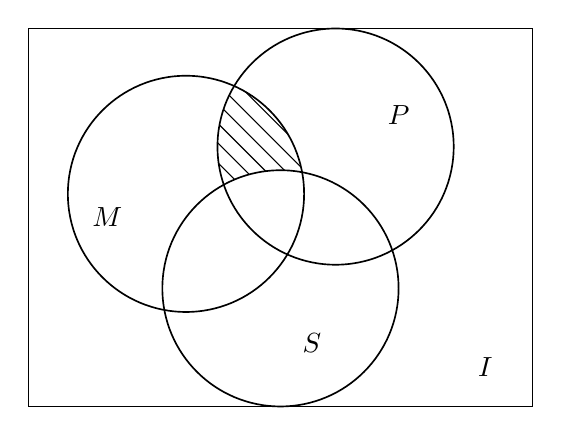
\begin{tikzpicture}[line width=.6pt,font=\normalsize]
  \coordinate (M) at (-1.2,0.3);
  \coordinate (P) at (0.7,0.9);
  \coordinate (S) at (0,-0.9);
  \draw (-3.2,-2.4) rectangle (3.2,2.4);
  \begin{scope}
    \clip (M) circle (1.5);
    \clip (P) circle (1.5);
    \foreach \x in {-4,-3.75,...,3.25} {\draw[line width=.4pt] (\x,2.4) -- (\x+4.8,-2.4);}
  \end{scope}
  \fill[white] (S) circle (1.5);
  \draw (M) circle (1.5);
  \draw (P) circle (1.5);
  \draw (S) circle (1.5);
  \node at (-2.2,0) {$M$};
  \node at (1.5,1.3) {$P$};
  \node at (0.4,-1.6) {$S$};
  \node at (2.6,-1.9) {$I$};
\end{tikzpicture}
